\section{Frozen transfer and modality comparisons}
\label{sec:late-transfer}
\cohortline{LABELED TRANSFER / 468 eligible queries / 32 development-exposed sequences / annotated ROI}

On the labeled transfer queries, PHASE-TTC had lower error than the earlier Garl adapter, but the RGB-only model remained stronger on average. The full error distribution reveals a mixed comparison with RGB: fusion had a lower empirical 95th percentile and more of the largest errors.

\subsection{Evaluation data and scoring}

This evaluation uses labeled EvTTC sequences and the earlier frozen Garl adapter.
Both differ from the 434-query competition experiment in
Section~\ref{sec:evttc-competition}.

We froze the final candidate before evaluating transfer on EvTTC, with no further fitting or checkpoint selection. We registered sixteen uniformly spaced query times in each of thirty-two sequences with compatible sensors and object annotations, and retained forty-six queries from the earlier evaluation. Removing four duplicates left 554 physical queries. Predictions were fixed before using TTC labels for scoring. The selected query times differ from those in the earlier 946- and 3,640-query H8 evaluations, including on shared sequences.

Each query received the nearest public TTC label within 50\,ms, with the earlier timestamp breaking ties. Forty queries had no label within that tolerance. We scored Historical46 and Extended-new separately, using 46 and 468 labeled queries. Their query identities are disjoint after duplicate removal, although all three Historical46 sequences also appear among the thirty-two Extended-new sequences. All retained TTC labels are positive.

Relative time error was defined as
\begin{equation}
\mathrm{RTE}=100\,\frac{|\widehat T-T|}{|T|},
\end{equation}
without clipping the signed nonzero target. Pooled summaries give each query equal weight; sequence-macro summaries give each physical sequence equal weight. We resample whole sequences for confidence intervals to preserve correlation between nearby query times. EvTTC had already informed development, so the evaluation is exploratory. Inputs also use annotated boxes, and temporal support differs: PHASE-TTC can use up to 650\,ms, while Garl uses two frames and event segments separated by 0.1\,s. Both use float32 tensors, but backend settings were not matched.

\begin{table}[H]
\centering\small
\caption{Frozen TRAIN40 transfer on \texttt{extended\_new}: 468 GT-valid queries, 32 sequences, positive TTC only, annotated ROI. Pooled metrics; lower is better. Source \evidence{L01}.}
\label{tab:late-transfer}
\begin{tabular}{lrrrr}
\toprule
\textbf{Model} & \textbf{MAE (s)} & \textbf{RTE (\%)} & \textbf{Median AE (s)} & \textbf{P95 AE (s)} \\
\midrule
Event context & 1.451 & 65.70 & 0.857 & 4.397 \\
Garl reproduced & 3.258 & 140.07 & 0.674 & 5.252 \\
Phase correction & 1.023 & 41.23 & 0.464 & 3.243 \\
RGB context & 1.015 & 38.56 & 0.408 & 3.799 \\
\bottomrule
\end{tabular}
\end{table}



\subsection{Average error and the RGB comparison}

PHASE-TTC's advantage over the earlier Garl full adapter extended across most scenes: it had lower sequence-mean RTE on twenty-six of thirty-two Extended-new sequences. Its pooled RTE was 41.23\% and MAE 1.023\,s (Table~\ref{tab:late-transfer}). Giving each sequence equal weight produced an RTE difference of $-94.83$ percentage points, with a 95\% bootstrap interval of $[-210.50,-14.49]$. The wide interval reflects substantial variation across scenes. \evidence{L01}

RGB alone remained the stronger model on average, with RTE of 38.56\% and MAE of 1.015\,s on the same queries. It also had lower pooled errors on Historical46. The RGB branch is therefore a more demanding reference for assessing the value of event fusion than the earlier Garl adapter.

The ordering changes farther into the saved error distribution. RGB also has the lower median error, while fusion's empirical 95th percentile is 3.24\,s against RGB's 3.80\,s (Figure~\ref{fig:transfer-tradeoff}). Fusion has lower sequence-mean RTE on fourteen of thirty-two sequences (Figure~\ref{fig:transfer-sequence}). \evidence{L01,L46}

\begin{figure}[H]
\centering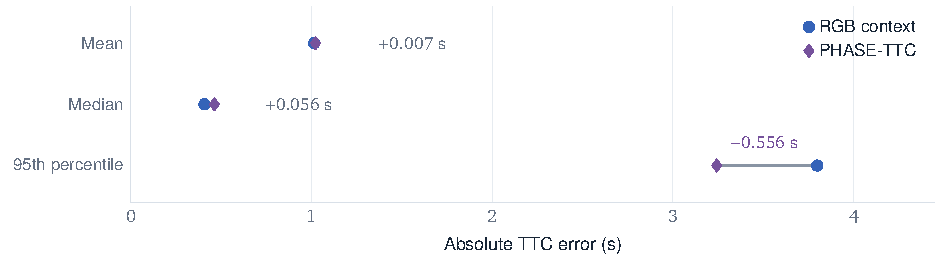
\includegraphics[width=0.94\linewidth]{figures/rev_transfer_pair.pdf}
\caption{\textbf{Absolute-error summaries for fusion and RGB.} Connected points compare the mean, median, and 95th percentile on the same 468 Extended-new queries. RGB has lower mean and median error; PHASE-TTC has a lower 95th percentile. Table~\ref{tab:revision-bootstrap} gives intervals for the paired differences.}
\label{fig:transfer-tradeoff}
\end{figure}

\subsection{Error exceedance and paired uncertainty}
The saved predictions contain fewer moderately large fusion errors but more extreme ones. PHASE-TTC has fewer absolute errors above 3\,s (29 versus 37) and 5\,s (9 versus 13), yet more above 10\,s (5 versus 2). Its maximum error reaches 32.5\,s, nearly twice RGB's 16.6\,s. We computed these threshold counts post hoc, retaining every eligible prediction in Figure~\ref{fig:transfer-exceedance}. \evidence{R01,L46}

\begin{figure}[htbp]
\centering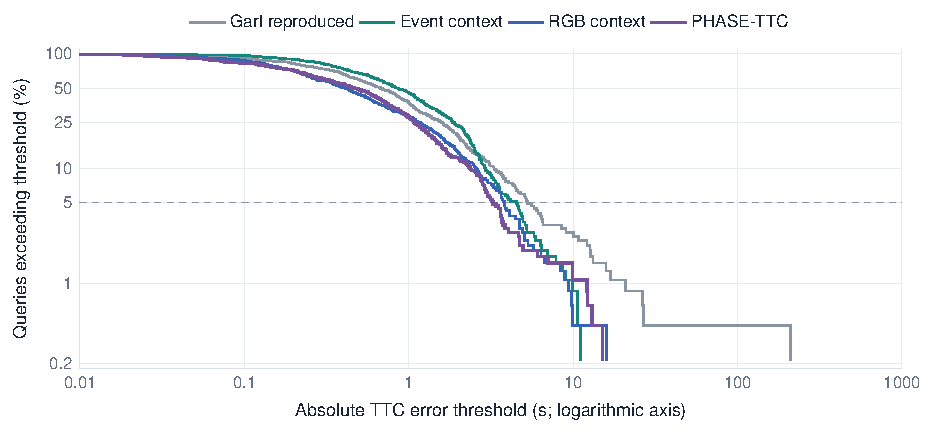
\includegraphics[width=\linewidth]{figures/rev_exceedance.pdf}
\caption{\textbf{Fraction of queries exceeding each absolute-error threshold.} Curves use all 468 labeled queries, with equal query weights and logarithmic axes. The dashed line marks 5\%. The plotted range includes the earlier Garl adapter's outlier above 600\,s. \evidence{R01,L46}}
\label{fig:transfer-exceedance}
\end{figure}

Resampling complete sequences gives a PHASE-minus-RGB p95 difference of $\RevisionPninetyfiveDelta$\,s, with a 95\% interval of $[\RevisionPninetyfiveLow,\RevisionPninetyfiveHigh]$\,s. The mean and median difference intervals also include zero. These exploratory intervals use 10,000 paired replicates, a fixed seed, and linear quantiles; they describe the saved models on sequences already used during development. Appendix~\ref{app:derived-transfer} provides the procedure, every sequence result, and two numerical cases selected post hoc. \evidence{R01}
\begin{table}[H]\centering\small
\caption{Paired differences in absolute error across 468 labeled queries from 32 sequences. Percentile intervals use 10,000 paired sequence resamples. \evidence{R01; derived from L46}}
\label{tab:revision-bootstrap}
\begin{tabular}{@{}lrrr@{}}\toprule
Metric & RGB (s) & PHASE-TTC (s) & Difference [95\% interval] (s)\\\midrule
Mean absolute error & 1.015 & 1.023 & $+0.007\;[-0.110,+0.129]$ \\
Median absolute error & 0.408 & 0.464 & $+0.056\;[-0.038,+0.145]$ \\
95th percentile & 3.799 & 3.243 & $-0.556\;[-1.126,+0.241]$ \\
\bottomrule\end{tabular}
\end{table}




\FloatBarrier
